\documentclass[11pt]{article}
\usepackage{cse216,hyperref}
% use the tikz package to draw automata
\usepackage{tikz}
\usetikzlibrary{arrows,positioning,automata}
\def\title{HW 5}
\begin{document}
\maketitle

\section*{Due November 3 at 3:00 pm}

\textbf{(1 question, 45 points total)}

\begin{qunlist}

  \q{45}{Transition systems}\\
  Consider the following closed transition system $M$:

  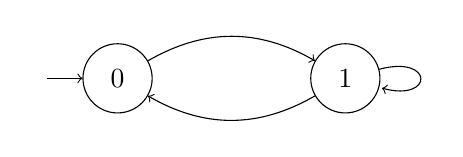
\begin{tikzpicture}[node distance=2cm]
    \node[state, initial, initial text=] (s0) {$0$};
    \node[state, right= of s0] (s1) {$1$};

    \path[->]
    (s0) edge[bend left] (s1)
    (s1) edge[bend left] (s0)
    (s1) edge[loop right] (s1);
  \end{tikzpicture}

  \begin{qparts}
  \item
    What are all runs of $M$ of length 3? (You can write them as triples of states.)

    \begin{answer}
      010

      011


    \end{answer}

  \item
    Let $\varphi$ be the trace property ``state 0 is visited infinitely many times''.
    Does $M \models \varphi$?
    Why or why not?

    \begin{answer}
      no. there exists a trace that goes \((0,1,1,1,1\dots)\) with only 1s that does not have state 0 infinitely many times.
    \end{answer}

  \item
    Let's run the BDD-based algorithm for computing the reachable states of $M$.
    First, write a BDD for the function $S_0(s)$ representing the initial states, which will also be the BDD $R_0(s)$ of states reachable in at most 0 steps.

    \begin{answer}
      since there are only 2 states, a single bit is enough to represent the states.

      \begin{equation}
        S_0(s)=\neg s
      \end{equation}

    \end{answer}

  \item
    Write a BDD for the function $\delta(s, s')$ representing the transition relation.

    \begin{answer}
      \begin{equation}
        \delta(s, s') = (\neg s \land s') \lor (s \land \neg s') \lor (s \land s')
      \end{equation}
    \end{answer}

  \item
    Write a BDD for the function $R_0(s) \land \delta(s, s')$.

    \begin{answer}
      \begin{equation}
        R_0(s) \land \delta(s, s') = \neg s \land (s \lor s') = (\neg s \land s) \lor (\neg s \land s') = 0 \lor (\neg s \land s') = \neg s \land s'
      \end{equation}
    \end{answer}

  \item
    Write a BDD for the function $\exists s. (S_0(s) \land \delta(s, s'))$ (which should only depend on $s'$).

    \begin{answer}
      \begin{equation}
        \exists s. (\neg s \land s') = (\neg 0 \land s') \lor (\neg 1 \land s') = (1 \land s') \lor (0 \land s') = s'
      \end{equation}
    \end{answer}

  \item
    Write a BDD for the function $R_1(s') = R_0(s) \lor \exists s. (S_0(s) \land \delta(s, s'))$.

    \begin{answer}
      \begin{equation}
        R_1(s') = \neg s' \lor s' = 1 \text{ (True)}
      \end{equation}

    \end{answer}

  \item
    What will happen in the next iteration of the algorithm?

    \begin{answer}
      A fixpoint is reached because $R_1$ covers all states ($0$ and $1$). The next iteration will yield $R_2 = R_1$, so the algorithm terminates with all states marked as reachable.
    \end{answer}
  \end{qparts}

\end{qunlist}
\end{document}
